\section{Introduction}
\begin{wrapfigure}[18]{r}{0.45\textwidth}
\vspace{-2em}
  \begin{center}
    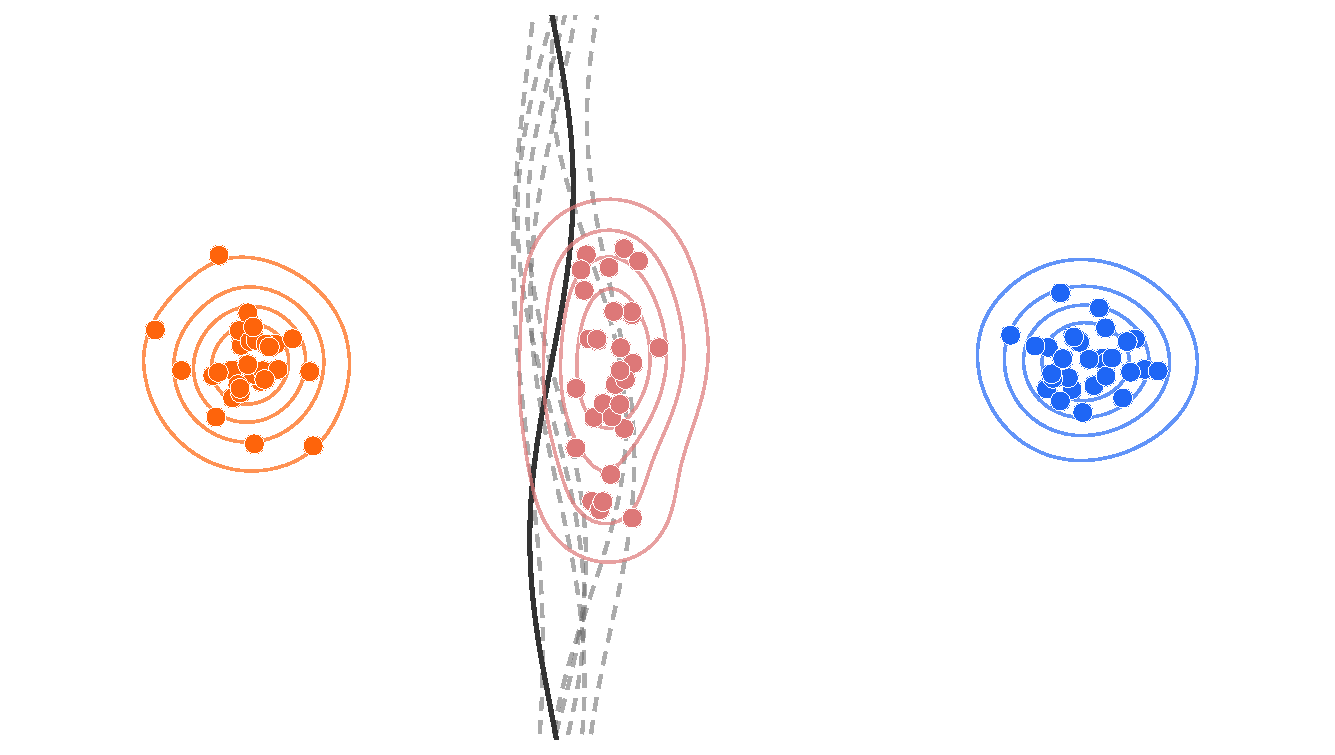
\includegraphics[trim={1.5cm 2cm 1.5cm 2cm},clip,width=\linewidth]{Figures/cf_sketch_proximal.pdf}
  \end{center}
  \caption{\textbf{Illustrative example of decision boundary shift.} A population of counterfactuals (pink) sits near a decision boundary (solid curve) separating two class distributions (orange and blue). Dashed lines indicate how the boundary's position could shift, illustrating why a counterfactual valid under the current boundary may become invalid under a shifted one.}
    \label{fig:robustness}
\end{wrapfigure}


Counterfactual explanations (CFs) help users identify changes that would alter a machine learning model's prediction. 
During the generation process, most methods assume a fixed model and data distribution; in deployment, however, the setting is considerably more dynamic~\citep{quionero2009dataset}. 
Evolving data distributions or policy changes cause retraining, and previously generated CFs might lose their validity in the new setting~\citep{rawal2020algorithmic}.
A counterfactual explanation that recommends actions to alter a model's prediction is only useful if the action still delivers the desired outcome for a model that might have been updated in between. 
When it does not, the recourse for a user, for example, an applicant told to raise their income by \$ 3000 to secure loan  approval, expires, undermining the trustworthiness and utility of CFs in dynamic environments (Figure~\ref{fig:robustness}).



This concern is not only at an individual level but also distributional. 
A bank, for instance, does not provide a single counterfactual but a population of them, one per rejected applicant. When the underlying data distribution shifts and the model is retrained, it is not only one CF but a fraction of the previously generated population that becomes invalid.
From an institutional perspective, the relevant object of robustness is not the individual CF but the distributional risk of invalidity across the entire generated population, a risk that instance-by-instance certification cannot control, since it never represents the population as an object of its own.





Current strategies aim to ensure that a counterfactual remains valid despite model updates. 
One line of work constrains these changes \emph{implicitly}, without directly modeling how the model might change: counterfactuals are optimized for high classification certainty~\citep{dutta2022robust,Hamman2023Robust, DBLP:conf/aaai/JiangL0T23}, training data is augmented with CFs~\citep{ferrario2022robustness}, or robustness is certified a posteriori under a Bayesian view over a user-specified pool of retrained models~\citep{stkepka2025counterfactual, duell2026provably}. 
Another line of work models the changes \emph{explicitly}, bounding against plausible parameter shifts for a single CF~\cite{upadhyay2021towards,kayastha2024learning,kyaw2025optimal, Marzari2024Rigorous,DBLP:conf/acml/JiangLL0T23}, including against a mixture of plausible future parameter distributions~\citep{DBLP:conf/iclr/NguyenBN23}. 
Two works come closer to a population view: \citet{bui2022counterfactual} jointly optimize a small per-instance set of CFs for joint validity under a shifted model, while \citet{nguyen2022robust} perturb the data distribution directly but still certify recourse one input at a time.
Neither treats the population generated across instances as the object of robustness.

% \begin{wrapfigure}[30]{r}{0.5\textwidth}
% \vspace{-2em}
%     \centering
%     \begin{subfigure}[b]{0.32\textwidth}
%         \centering
%         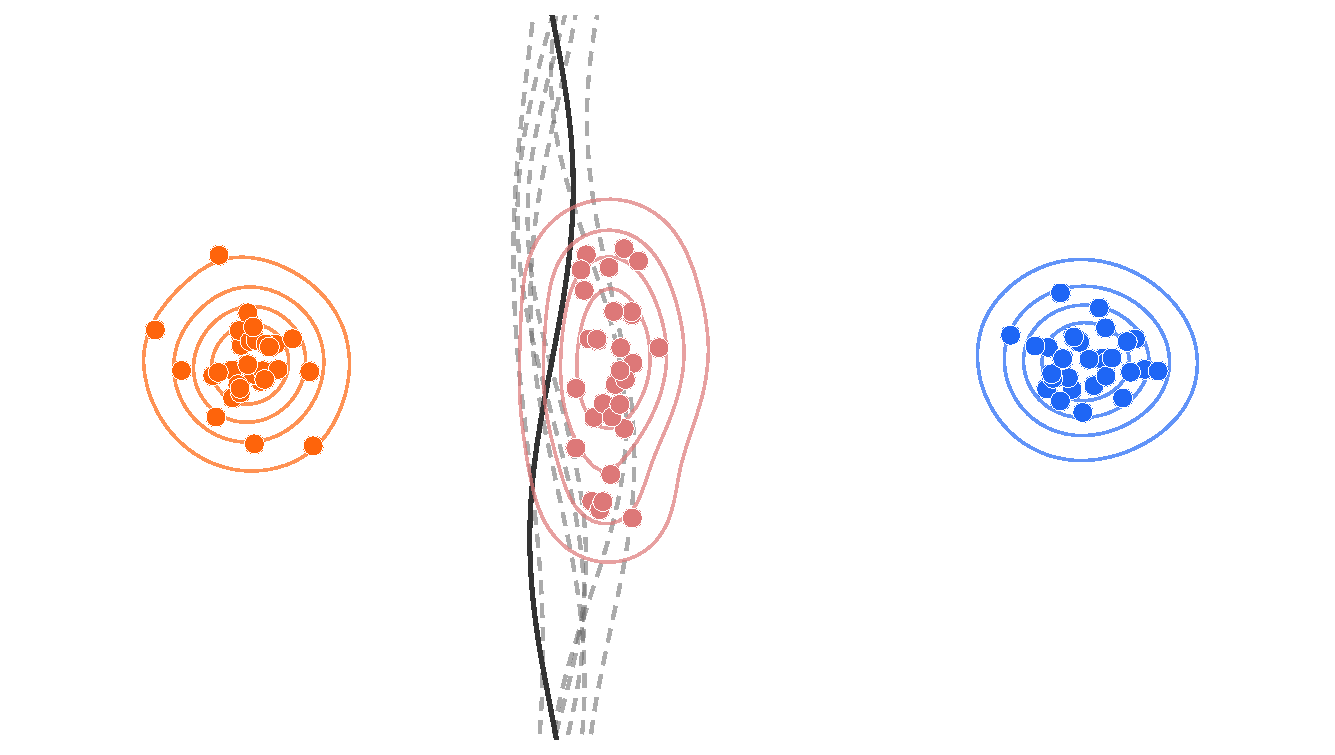
\includegraphics[trim={1.5cm 2cm 1.5cm 2cm},clip,width=\linewidth]{Figures/cf_sketch_proximal.pdf}
%         \caption{Proximal CFs.}
%         \label{fig:proximal}
%     \end{subfigure}
    
%     \vspace{4pt}
    
%     \begin{subfigure}[b]{0.32\textwidth}
%         \centering
%         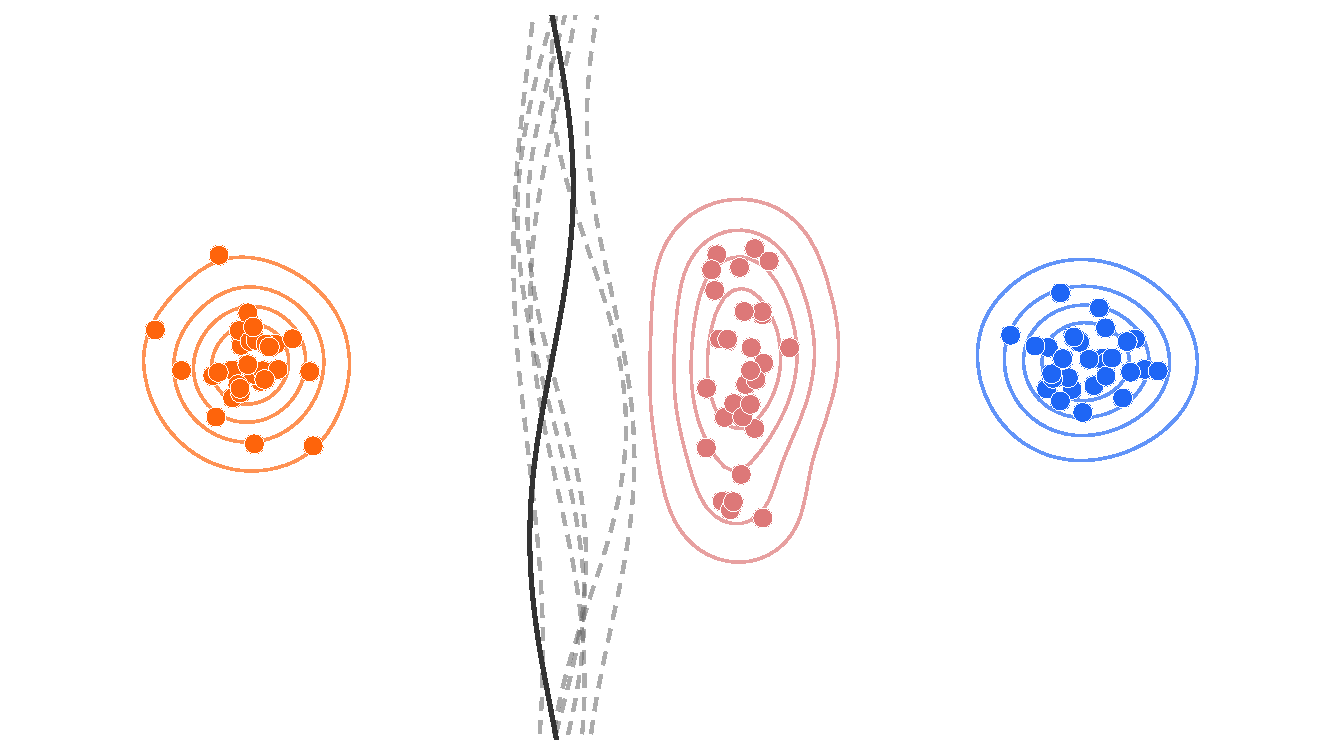
\includegraphics[trim={1.5cm 2cm 1.5cm 2cm},clip,width=\linewidth]{Figures/cf_sketch_robust.pdf}
%         \caption{Robust CFs.}
%         \label{fig:robust}
%     \end{subfigure}
    
%     \vspace{4pt}
    
%     \begin{subfigure}[b]{0.32\textwidth}
%         \centering
%         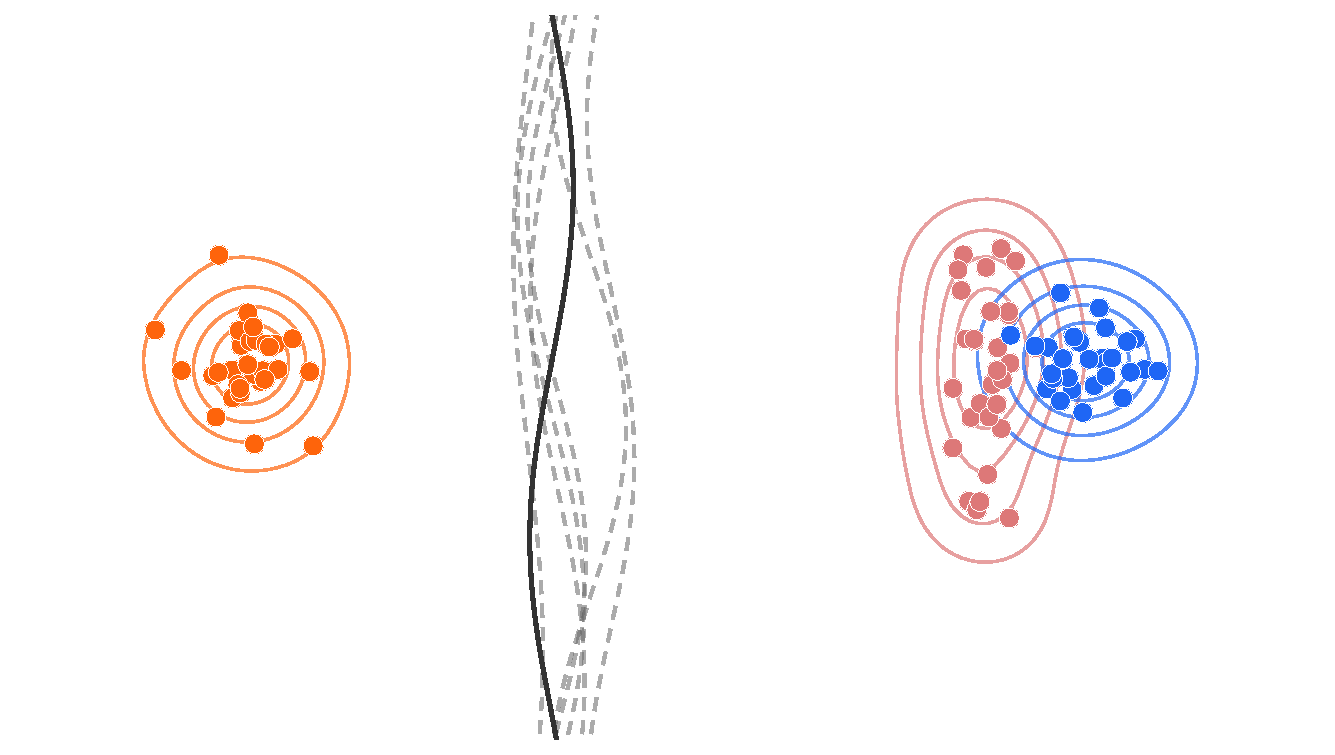
\includegraphics[trim={1.5cm 2cm 1.5cm 2cm},clip,width=\linewidth]{Figures/cf_sketch_plausible.pdf}
%         \caption{Plausible CFs.}
%         \label{fig:plausible}
%     \end{subfigure}
    
%     \caption{\textbf{Counterfactual types under decision boundary shift.} Counterfactuals (pink) are generated near a decision boundary (solid curve) separating two class distributions (orange and blue). Dashed lines show possible boundary shifts. \textbf{(a) Proximal} CFs stay close to the original boundary and become invalid under shift. \textbf{(c) Plausible} CFs lie within the target class distribution, by disregarding proximity, they often require larger and less actionable changes than necessary. \textbf{(b) Robust} CFs stay as close as possible to the original input, combining actionability of (a) with the robustness of (c). }
%     \label{fig:overall}
% \end{wrapfigure}

We address this gap with \textsc{LIFT-CF}, a post-hoc distributional refinement that treats the population of CFs produced by any CF generator as a distribution to be moved, via a calibrated Wasserstein lens anchored to the target class and the generator's output, toward a region of lower worst-case future invalidity.
Our main contributions are:
\begin{itemize}
    \item We introduce the \emph{CF-induced Wasserstein lens}, an ambiguity set of target-side distributions close to the observed target class and generator output, giving a worst-case notion of distributional lens risk that a refined CF population can be optimized against.
    \item We show that minimizing a tractable convex relaxation of this worst-case risk reduces to a one-dimensional Wasserstein barycentric family between the CF and target distributions, and select the deployed refinement by directly evaluating robustness to adversarial retraining shifts on held-out data, with a matching Lipschitz stability guarantee bounding the resulting finite-grid search error.
    \item We realize the calibrated refinement via optimal transport and show empirically that it \textcolor{latte_maroon}{experiments?}
\end{itemize}